\documentclass{article}%
\usepackage[T1]{fontenc}%
\usepackage[utf8]{inputenc}%
\usepackage{lmodern}%
\usepackage{textcomp}%
\usepackage{lastpage}%
\usepackage{amsmath}%
\usepackage{qcircuit}%
\usepackage{graphicx}%
%
%
%
\begin{document}%
\normalsize%
\section{3{-}SAT Solution Report}%
\label{sec:3{-}SATSolutionReport}%
This report contains solutions for the 3{-}SAT problem reduced from original independent set problem,executed on Qiskit Aer Simulators.\newline%
%
Report generated on: 2024{-}11{-}15 15:16:24%
\subsection{3{-}SAT Formula}%
\label{subsec:3{-}SATFormula}%
The 3{-}SAT formula consists of the following clauses:\newline%
%
\[ (\neg x_1 \lor \neg x_2) \land (\neg x_1 \lor \neg x_3) \land (\neg x_2 \lor \neg x_3) \land (\neg x_2 \lor \neg x_4) \land (x_2 \lor x_3 \lor x_1) \land (\neg x_5 \lor x_1 \lor x_3) \land (x_5 \lor \neg x_1) \land (x_5 \lor \neg x_3) \land (x_5 \lor x_4 \lor x_2) \land (x_1 \lor x_2 \lor x_3) \land (x_2 \lor x_4) \]

%
\subsection{QUBO Matrix Visualization}%
\label{subsec:QUBOMatrixVisualization}%
Converted QUBO matrix visualization:\newline%
%
$\begin{bmatrix}
-4.0 & 3.0 & 4.0 & 0.0 & -1.0 & 0.0 & 0.0 & 0.0 & 0.0 & 1.0 & 1.0 & 0.0 & 0.0 & 0.0 & 1.0\\0.0 & -7.0 & 3.0 & 4.0 & 1.0 & 0.0 & 0.0 & 0.0 & 0.0 & 1.0 & 0.0 & 0.0 & 0.0 & 1.0 & 1.0\\0.0 & 0.0 & -4.0 & 0.0 & -1.0 & 0.0 & 0.0 & 0.0 & 0.0 & 1.0 & 1.0 & 0.0 & 0.0 & 0.0 & 1.0\\0.0 & 0.0 & 0.0 & -3.0 & 1.0 & 0.0 & 0.0 & 0.0 & 0.0 & 0.0 & 0.0 & 0.0 & 0.0 & 1.0 & 0.0\\0.0 & 0.0 & 0.0 & 0.0 & -2.0 & 0.0 & 0.0 & 0.0 & 0.0 & 0.0 & 1.0 & 0.0 & 0.0 & 1.0 & 0.0\\0.0 & 0.0 & 0.0 & 0.0 & 0.0 & 0.0 & 0.0 & 0.0 & 0.0 & 0.0 & 0.0 & 0.0 & 0.0 & 0.0 & 0.0\\0.0 & 0.0 & 0.0 & 0.0 & 0.0 & 0.0 & 0.0 & 0.0 & 0.0 & 0.0 & 0.0 & 0.0 & 0.0 & 0.0 & 0.0\\0.0 & 0.0 & 0.0 & 0.0 & 0.0 & 0.0 & 0.0 & 0.0 & 0.0 & 0.0 & 0.0 & 0.0 & 0.0 & 0.0 & 0.0\\0.0 & 0.0 & 0.0 & 0.0 & 0.0 & 0.0 & 0.0 & 0.0 & 0.0 & 0.0 & 0.0 & 0.0 & 0.0 & 0.0 & 0.0\\0.0 & 0.0 & 0.0 & 0.0 & 0.0 & 0.0 & 0.0 & 0.0 & 0.0 & -2.0 & 0.0 & 0.0 & 0.0 & 0.0 & 0.0\\0.0 & 0.0 & 0.0 & 0.0 & 0.0 & 0.0 & 0.0 & 0.0 & 0.0 & 0.0 & -1.0 & 0.0 & 0.0 & 0.0 & 0.0\\0.0 & 0.0 & 0.0 & 0.0 & 0.0 & 0.0 & 0.0 & 0.0 & 0.0 & 0.0 & 0.0 & 0.0 & 0.0 & 0.0 & 0.0\\0.0 & 0.0 & 0.0 & 0.0 & 0.0 & 0.0 & 0.0 & 0.0 & 0.0 & 0.0 & 0.0 & 0.0 & 0.0 & 0.0 & 0.0\\0.0 & 0.0 & 0.0 & 0.0 & 0.0 & 0.0 & 0.0 & 0.0 & 0.0 & 0.0 & 0.0 & 0.0 & 0.0 & -2.0 & 0.0\\0.0 & 0.0 & 0.0 & 0.0 & 0.0 & 0.0 & 0.0 & 0.0 & 0.0 & 0.0 & 0.0 & 0.0 & 0.0 & 0.0 & -2.0
\end{bmatrix}$

%
\subsection{QAOA Configurations}%
\label{subsec:QAOAConfigurations}%
QAOA is configured with the following parameters:\newline%
%
\begin{itemize}%
\item%
Layers: \(3\)%
\item%
Maximizer Hamiltonian: Standard mixing Hamiltonian \( H_M = \sum_{i} X_i \)%
\item%
Classical Optimizer: Powell's Method%
\item%
Maximum Iterations: \(500\)%
\item%
Initialization: \(\gamma = 2\pi\), \(\beta = \pi\)%
\end{itemize}

%
\subsection{QAOA Solution}%
\label{subsec:QAOASolution}%
The most probable solution obtained from the QAOA optimization is as follows:\newline%
%
\begin{itemize}%
\item Variable \( x_1 \) is set to true%
\item Variable \( x_2 \) is set to false%
\item Variable \( x_3 \) is set to true%
\item Variable \( x_4 \) is set to false%
\item Variable \( x_5 \) is set to true%
\item Variable \( x_6 \) is set to false%
\item Variable \( x_7 \) is set to true%
\item Variable \( x_8 \) is set to false%
\item Variable \( x_9 \) is set to true%
\item Variable \( x_10 \) is set to false%
\item Variable \( x_11 \) is set to false%
\item Variable \( x_12 \) is set to true%
\item Variable \( x_13 \) is set to false%
\item Variable \( x_14 \) is set to true%
\item Variable \( x_15 \) is set to false%
\end{itemize}

%


\begin{figure}[h!]%
\centering%
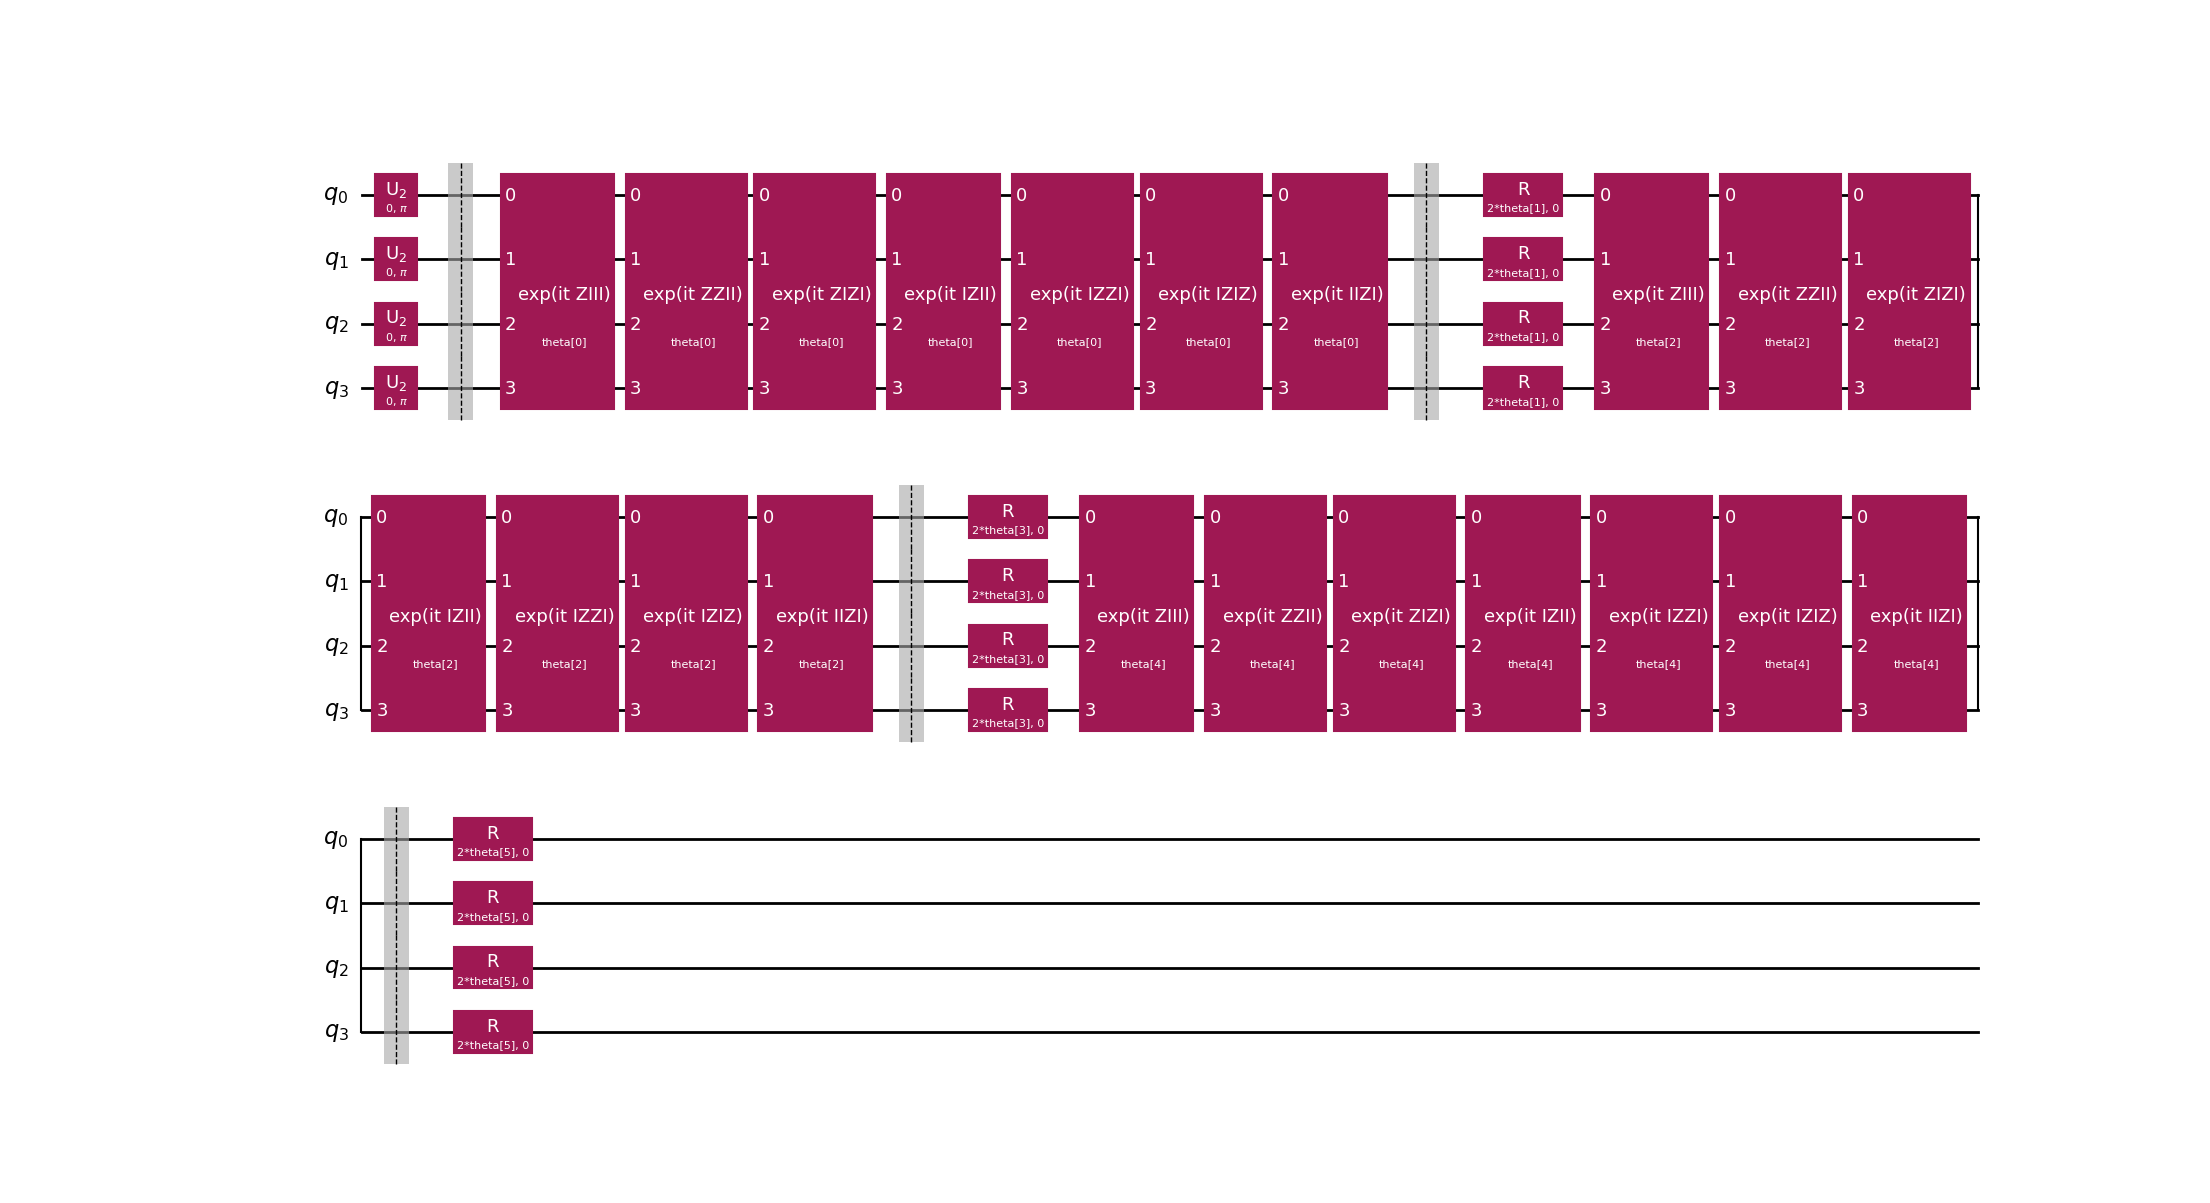
\includegraphics[width=120px]{quantum_circuit_qaoa.png}%
\caption{QAOA Circuit Visualization}%
\end{figure}

%
\subsection{VQE Configurations}%
\label{subsec:VQEConfigurations}%
VQE is configured with the following parameters:\newline%
%
\begin{itemize}%
\item%
Layers: \(3\)%
\item%
Ansatz: Two-local%
\item%
Classical Optimizer: Powell's Method%
\item%
Maximum Iterations: \(500\)%
\item%
Initialization: \(\theta = \pi\)%
\end{itemize}

%
\subsection{VQE Solution}%
\label{subsec:VQESolution}%
The most probable solution obtained from the VQE optimization is as follows:\newline%
%
\begin{itemize}%
\item Variable \( x_1 \) is set to false%
\item Variable \( x_2 \) is set to false%
\item Variable \( x_3 \) is set to true%
\item Variable \( x_4 \) is set to true%
\item Variable \( x_5 \) is set to true%
\item Variable \( x_6 \) is set to false%
\item Variable \( x_7 \) is set to true%
\item Variable \( x_8 \) is set to false%
\item Variable \( x_9 \) is set to false%
\item Variable \( x_10 \) is set to true%
\item Variable \( x_11 \) is set to false%
\item Variable \( x_12 \) is set to false%
\item Variable \( x_13 \) is set to false%
\item Variable \( x_14 \) is set to true%
\item Variable \( x_15 \) is set to true%
\end{itemize}

%


\begin{figure}[h!]%
\centering%
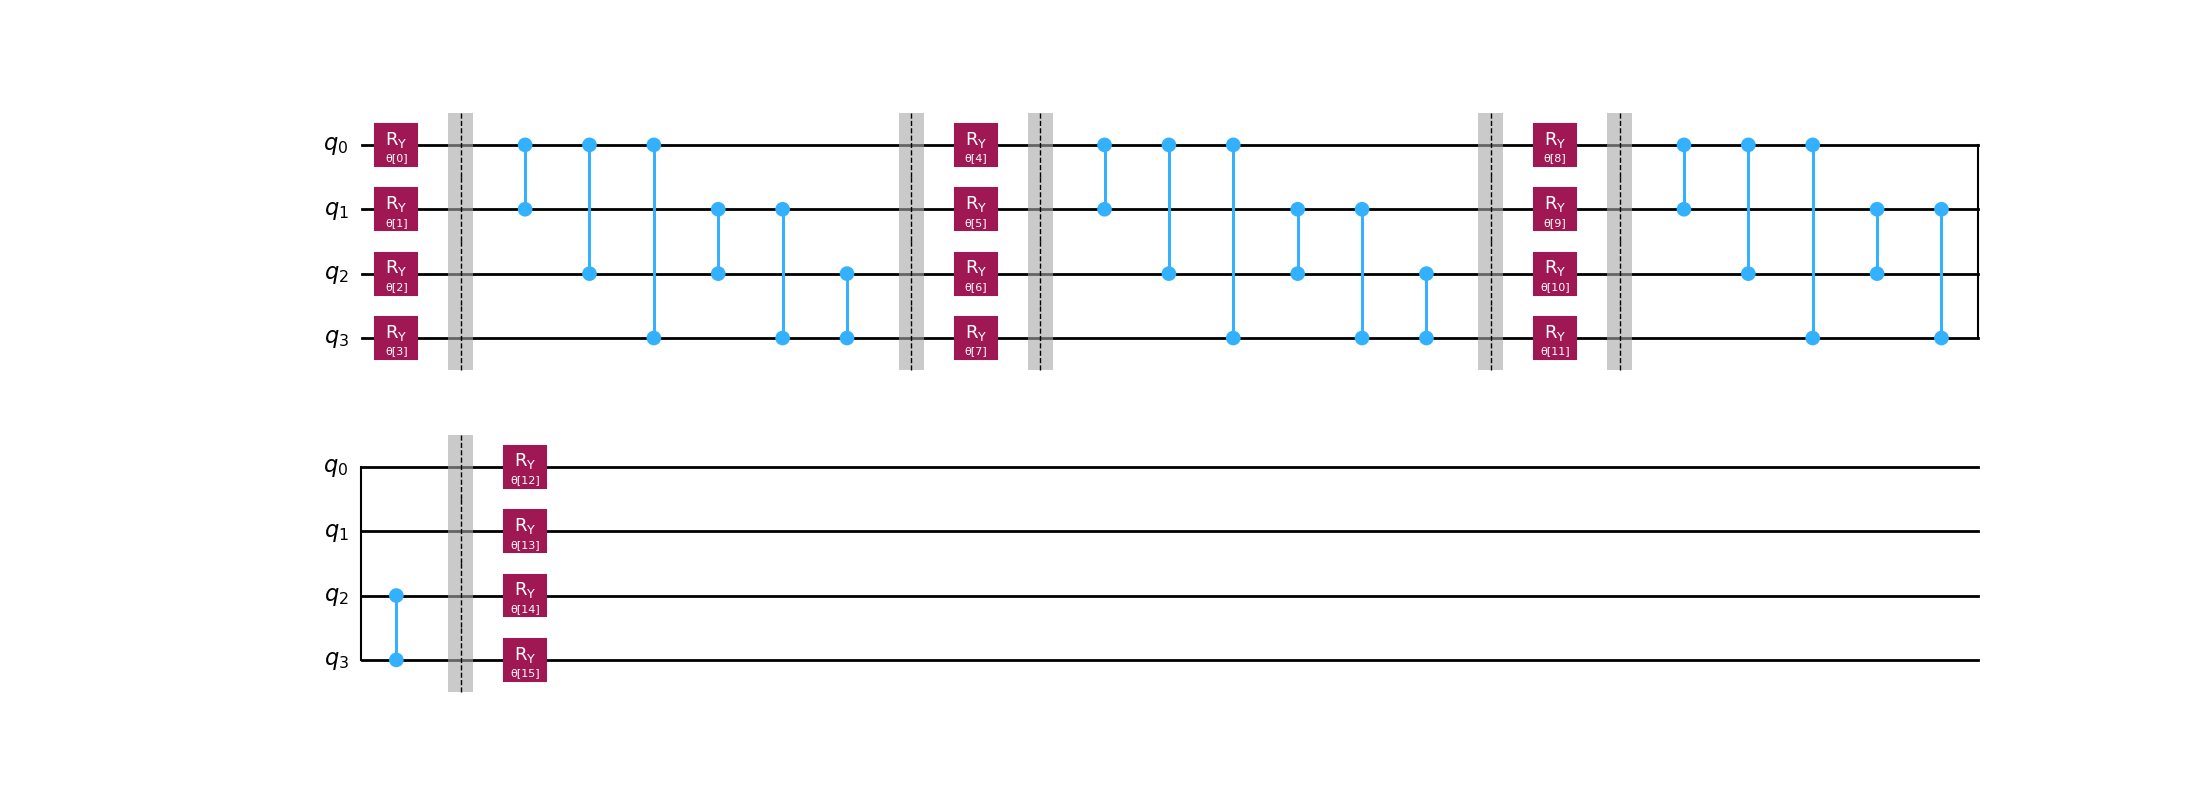
\includegraphics[width=120px]{quantum_circuit_vqe.png}%
\caption{VQE Circuit Visualization}%
\end{figure}

%
\subsection{Grover's algorithm Configurations}%
\label{subsec:GroversalgorithmConfigurations}%
Grover is configured with the following parameters:\newline%
%
\begin{itemize}%
\item%
Iterations: \(1\)%
\end{itemize}

%
\subsection{Grover's Algorithm Solution}%
\label{subsec:GroversAlgorithmSolution}%
The most probable solution obtained from the Grover optimization is as follows:\newline%
%
\begin{itemize}%
\item Variable \( x_1 \) is set to false%
\item Variable \( x_2 \) is set to false%
\item Variable \( x_3 \) is set to true%
\item Variable \( x_4 \) is set to false%
\item Variable \( x_5 \) is set to false%
\end{itemize}

%


\begin{figure}[h!]%
\centering%
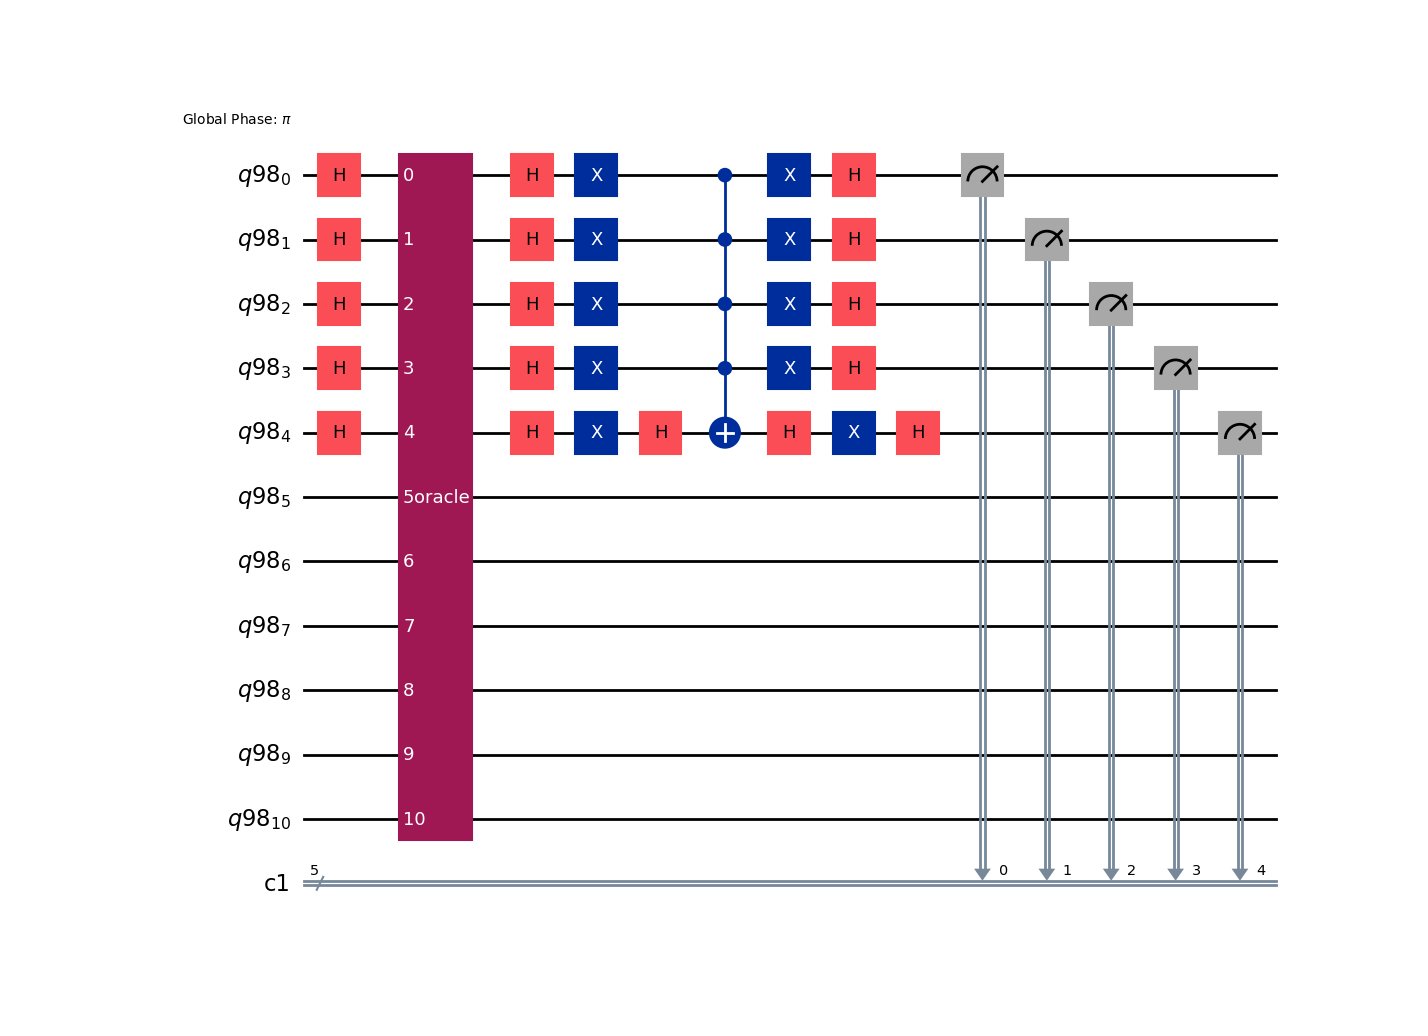
\includegraphics[width=120px]{quantum_circuit_grover.png}%
\caption{Grover's Algorithm Circuit Visualization}%
\end{figure}

%
\end{document}